\documentclass{exam}
\usepackage[utf8]{inputenc}
\usepackage{color}
\usepackage{amsmath}
\usepackage[italian]{babel}
\usepackage{comment}
\usepackage{graphicx}
\usepackage[siunitx]{circuitikz}
\newcommand{\splitcell}[2][c]{%
  \begin{tabular}[c]{@{}c@{}}\strut#2\strut\end{tabular}%
}
\usepackage{natbib}
\usepackage{listings}
\usepackage{xparse}
\usepackage{hyperref}
\usepackage{float}
\usepackage{tcolorbox}

\NewDocumentCommand{\codeword}{v}{%
\texttt{\textcolor{blue}{#1}}%
}
\usepackage{pgfplots}
\pgfplotsset{compat = newest}
\usepackage{chngcntr}
\counterwithin{table}{section}
\counterwithin{figure}{section}

\usepackage{listings}
\usepackage{xcolor}

\definecolor{codegreen}{rgb}{0,0.6,0}
\definecolor{codegray}{rgb}{0.5,0.5,0.5}
\definecolor{codepurple}{rgb}{0.58,0,0.82}
\definecolor{backcolour}{rgb}{0.95,0.95,0.92}

\lstdefinestyle{mystyle}{
    backgroundcolor=\color{backcolour},   
    commentstyle=\color{codegreen},
    keywordstyle=\color{magenta},
    numberstyle=\tiny\color{codegray},
    stringstyle=\color{codepurple},
    basicstyle=\ttfamily\footnotesize,
    breakatwhitespace=false,         
    breaklines=true,                 
    captionpos=b,                    
    keepspaces=true,                 
    numbers=left,                    
    numbersep=5pt,                  
    showspaces=false,                
    showstringspaces=false,
    showtabs=false,                  
    tabsize=2
}

\lstset{style=mystyle}

\begin{document}

\newcommand{\Exjobbsnummer}[1]{
	\begin{tikzpicture}[overlay, remember picture]
		\path (current page.north east) ++(-1,-1) node[below left] {{\small #1}};
	\end{tikzpicture}
}

\newcommand{\Examensjobbspoang}[1]{
	\begin{tikzpicture}[overlay, remember picture]
		\path (current page.north east) ++(-1,-1.5) node[below left] {{\normalsize \scshape Examensarbete #1 HP}};
	\end{tikzpicture}
}

\newcommand{\datum}[1]{
	\begin{tikzpicture}[overlay, remember picture]
		\path (current page.north east) ++(-1,-2.0) node[below left] {{\normalsize #1}};
	\end{tikzpicture}}

\newcommand{\storlitentitel}[2]{
\center
\rule[0.2cm]{13cm}{0.1cm}
{ \huge \bfseries #1}\\[0.4cm] % Title of your document
{\Large \slshape #2}\\[0.4cm]
\rule[0.2cm]{13cm}{0.1cm}\\[3cm]

}

\newcommand{\Namn}[2]{
	\begin{minipage}{0.5\textwidth}
		\normalsize
		\centering
		#1 \textsc{#2}\\
	\end{minipage}\\
}

\newcommand{\LoggaSwe}{
	\textsc{\Huge Laboratorio \\[0.3cm] di Internet}\\[0.7cm]
	
\includegraphics[scale=.06]{polito_logo_2021_blu.jpg}\\[1.5cm]
}

\newcommand{\LoggaEng}{
	\textsc{\Huge Uppsala University}\\[0.7cm]
	\includegraphics[scale=.1]{Uppsala_University_seal_svg.png}\\[0.5cm]
}


% -----------------------------------------------
%           HÄR BÖRJAR TITELSIDAN
%------------------------------------------------
\begin{titlepage}

	\center

	%-------------------------------------------------
	%	INFORMATION ATT FYLLA I
	%-------------------------------------------------
	\Exjobbsnummer{Anno Accademico 2021/2022}
	%\datum{2021/2022}

	\LoggaSwe
	% \LoggaEng - Byt till engelska


	\storlitentitel{\\Report II}{Stima di velocità tramite ping}

	\Large Gruppo 14\\
	\Namn{guest1}{(s000000)}
	\Namn{Alessandro Ciullo}{(s310023)}
	\Namn{guest3}{(s000000)}



	\vfill

\end{titlepage}

%\title{%
%  \textbf{LABORATORIO DI INTERNET} \\
% \textbf{ \large REPORT I: CONNECTIVITY CHECK - ADVANCED PING}}

%\author{ Andreas Brummer(s270332)  Alessandro Ciullo(s269589)  \\Andrea %Scamporrino(s270971)}
%\date{}

% \begin{figure}
%   \centering
%   
\includegraphics[scale = 0.10]{polito_logo_2021_blu.jpg}
%\end{figure}
%\maketitle

\pagebreak
\section{Configurazione di rete}

Nell'effettuare i test é stata usata la seguente configurazione di rete:

\begin{table}[h!]
	\centering
	\begin{tabular}{|c|c|}
		\hline
		Indirizzo di rete      & 172.16.14.0     \\
		\hline
		Indirizzo di broadcast & 172.16.14.63    \\
		\hline
		NetMask                & 255.255.255.192 \\
		\hline
	\end{tabular}
	%\caption{Configurazione di rete}
	\label{tab:testbed}
\end{table}

\begin{table}[h!]
	\centering
	\begin{tabular}{|c|c|}
		\hline
		Nome host & Indirizzo IP   \\
		\hline
		H1        & 172.16.14.1/26 \\
		\hline
		H2        & 172.16.14.2/26 \\
		\hline
	\end{tabular}
	\caption{Configurazione di rete}
	\label{tab:testbed}
\end{table}

\section{Considerazioni sui parametri e le configurazioni utilizzate}
Nei vari scenari analizzati abbiamo utilizzato i 2 computer fissi del laboratorio collegati alla rete tramite cavo ethernet. Inoltre, abbiamo utilizzato degli adattatori usb-ethernet per la connessione perchè senza di essi la scheda di rete del computer svolge delle operazioni aggiuntive che interferiscono con i test svolti.
\subsection{RTT}
Nei vari calcoli del RTT si ipotizzerà che sia i tempi di elaborazione che i tempi di propagazione siano trascurabili. Le formule reali dovrebbero essere del tipo
\begin{equation}
	RTT_{reale} = RTT_{T_{TX}} + \eta
\end{equation}
Il primo termine rappresenta la somma di tutti i tempi di trasmissione, mentre il secondo indica un effetto di rumore dato dai tempi di elaborazione, propagazione e anche da altri fenomeni non deterministici
Per minimizzare il contributo di $\eta$ teniamo conto, in ciascuno dei test, del RTT minimo, misurato al variare della dimensione dei pacchetti inviati.. 
\subsection{Frammentazione}
Quando comunichiamo attraverso un canale ethernet la Maximum Transmission Unit (MTU) è di 1500 byte. Per ovviare a questo limite il protocollo IP, consapevole della MTU del livello di collegamenti dati su cui si appoggia, svolge un'operazione chiamata "frammentazione". L'IP fragmentation scompone le SDU in unità più piccole adatte alla trasmissione sul canale, e utilizza i campi "Fragment offset", "Don't Fragment" e "More Fragments" per permettere ai dispositivi di livello di rete di riassemblare il pacchetto alla loro ricezione.
Il fenomeno della frammentazione ha alcune importanti ripercussioni sul comportamento del RTT e della capacità al variare di S durante l'inoltro di pacchetti sulla rete internet.
Nel momento in cui un nuovo frammento viene generato il numero di dati da trasmettere dall'host incrementa in maniera non lineare: come mostrato in figura \ref{fig:StoD} prima si verifica un salto e in seguito un plateau che perdura finchè viene aggiunto del padding (necessario al raggiungimento del minimum frame size) al nuovo pacchetto.


\subsection{Calcolo di D(S)}
\begin{figure}[H]
	\centering
	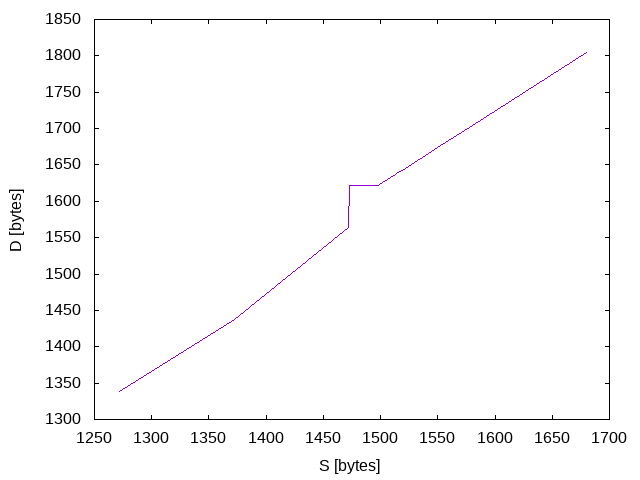
\includegraphics[scale = 0.75]{StoD.png}
	\caption{Grafico S-D}
	\label{fig:StoD}
\end{figure}
Per calcolare la corrispondenza tra i dati di livello applicazione(S) e quelli di livello fisico(D) si usa la seguente formula:
\begin{equation}
    \begin{cases}
        D(S) = S + H_{IP} + H_{ICMP} + H_{ETHERNET} , S \not\in [1473 + n \cdot 1472 ,n \cdot 1497+ n \cdot 1472], n \in \mathbf{N} \\
        D(S) = S + H_{IP} + H_{ICMP} + H_{ETHERNET}+ 46- (((S+8) \% 1480)+  H_{IP}) , S \in [1473 + n \cdot 1472 ,n \cdot 1497+ n \cdot 1472], n \in \mathbf{N} \\
        H_{IP} = 20\\
        H_{ICMP} = 8\\
        H_{ETHERNET} = 38
    \end{cases}
\end{equation}
\section{Host collegati direttamente tramite cavo ethernet}
In questa sezione analizziamo lo scenario in cui i due host H1 e H2 sono collegati in maniera diretta mediante un cavo Ethernet. Il modello utilizzato è semplice poichè $RTT = 2 \cdot T_{TX} =\dfrac{2 D}{C}$. Ricaviamo quindi che \begin{equation}\label{cap1}
	C = \dfrac{2D}{RTT}
\end{equation}.

 \begin{figure}[H]
	\centering
	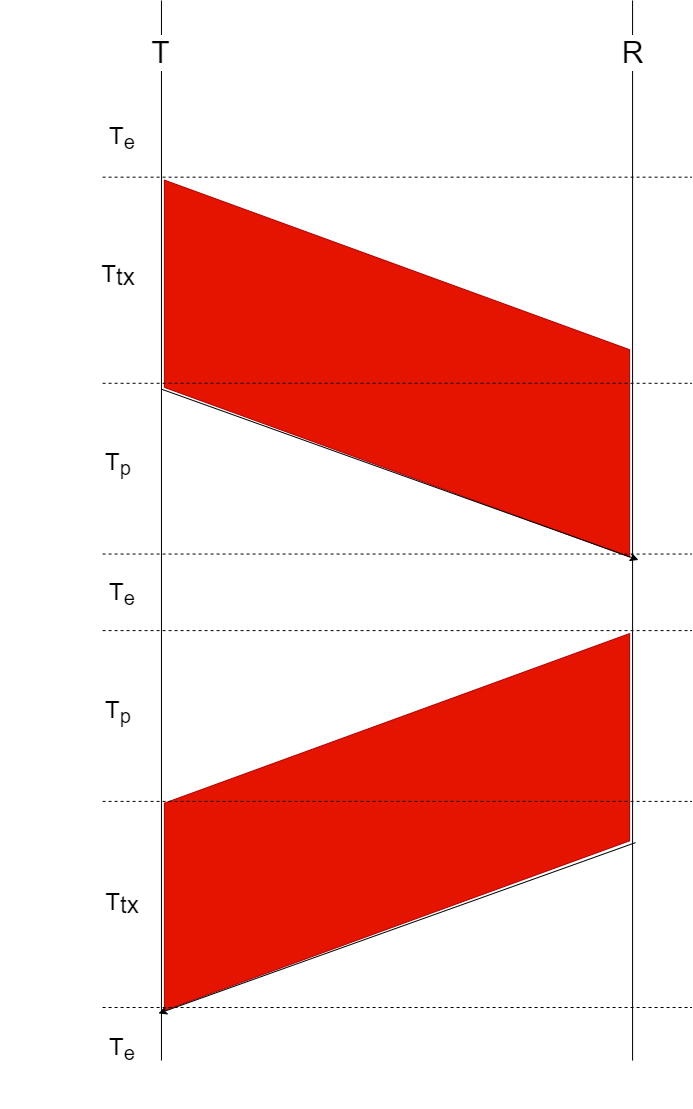
\includegraphics[scale = 0.26]{Grafico2.png}
	\caption{Schema invio diretto pacchetto}
	\label{fig:GrafnoSwitch}
\end{figure}

\subsection{Velocità: 10Mb/s}\label{10NS}
Abbiamo imposto la velocità di trasmissione sul canale a 10Mb/s Full Duplex eseguendo il seguente comando su uno dei due host.
\begin{lstlisting}
sudo ethtool -s eth0 speed 10 duplex full autoneg on
\end{lstlisting}
Attraverso il processo di auto-negoziazione viene impostata la velocità su entrambi gli host.\\

In figura \ref{fig:2.1RTT} il RTT teorico è messo a confronto con il RTT misurato con l'ausilio dello script \ref{fig:ScriptPing}.Essendo la velocità di trasferimento relativamente bassa, i tempi di elaborazione e propagazione diventano trascurabili rispetto al tempo di trasmissione e perciò ne consegue un comportamento reale estremamente simile a quello teorico. Seppur difficile da notare, per via della scala sulle ascisse molto ampia, è importante prestare attenzione al comportamento nell'intorno dei punti di frammentazione: il RTT compie un salto verso l'alto ad ogni frammentazione causato dal repentino aumento di D, e resta costante per il "periodo di padding" che consegue, continua poi il suo andamento lineare fino al prossimo punto di frammentazione.

In figura \ref{fig:2.1Speed} è invece riportato il grafico della capacità sul canale calcolata mediante l'equazione \ref{cap1}. L'andamento ottenuto è del tipo $C = 10*(1 - e^{-S})[Mbps]$ e come potevamo immaginare per $S\to\infty$ la capacità tende al valore negoziato tra i due host. In corrispondenza dei punti di frammentazione abbiamo un comportamento difficile da analizzare a causa di fattori fuori dalla nostra comprensione (tempi di elaborazione, operazioni svolte dalla scheda di rete ecc.) e abbiamo perciò potuto solo avanzare delle ipotesi:
%\begin{tcolorbox}
Come mostrato in appendice la capacità aumenta repentinamente nel primo Byte successivo alla frammentazione e poi decresce per un breve intervallo; al termine del fenomeno la funzione riassume il suo andamento naturale fino al successivo punto di frammentazione.

Tenendo conto della formula $C = D/{(2T_{TX}(D) +\eta)}$ e del fatto che il tempo di trasmissione vari in maniera lineare in funzione di D, possiamo ipotizzare che ad un aumento improvviso di D il contributo del termine $\eta$ si riduca e ne consegua un brusco aumento di C. Abbiamo, inoltre, immaginato che il successivo andamento decrescente avvenga nell'intervallo di padding e che sia causato dall'aumento dei tempi di elaborazione: seppur il valore D non cambi i dati elaborati a livello applicazione aumentano generando dei costi computazionali; l'inserimento del padding, invece, è fatto in maniera efficiente dalla scheda di rete e non comporta costi addizionali. Ne consegue perciò un andamento locale decrescente.
%\end{tcolorbox}


\subsection{Velocià: 100Mb/s}
Quando impostiamo una velocità più alta notiamo che le misure diventano molto più imprecise, questo accade perché l'impatto del termine $\eta$ di cui abbiamo parlato in precedenza è molto maggiore. Possiamo pensare che l'offset che notiamo ($\simeq 0,5 ms$) sia dovuto proprio al rumore ed in particolare al tempo di elaborazione. In questo caso i frammenti sono pochi (massimo 5), ma in realtà l'offset aumenta impercettibilmente all'aggiunta di ogni frammento(perché aumenta il tempo di elaborazione). La non linearità del RTT misurato probabilmente è dovuta ai termini casuali che compongono $\eta$.

La capacità, mostrata in figura \ref{fig:2.2Speed}, ha  un andamento generale del tipo $C = 100*(1 - e^{-S})[Mbps]$, ed in presenza di frammentazione si comporta in maniera simile al caso mostrato al punto \ref{10NS}, a meno di una piccola differenza: questa volta l'incremento repentino di C è meno evidente e prevale l'andamento decrescente nell'intorno dei punti di frammentazione. Possiamo attribuire la causa di questo fenomeno alla più alta velocità di trasmissione, che implica una capacità meno sensibile alle piccole variazioni di D. L'aumento dei costi computazionali è invece indipendente dal bit-rate e perciò l'andamento decrescente nell'intervallo di padding non è trascurabile.


\section{Host collegati tramite uno switch}
In questo caso entrambi gli host sono connessi attraverso uno switch che fa uso della tecnica di commutazione "Store and Forward": un pacchetto per essere inviato deve prima essere interamente ricevuto e memorizzato. 

Quando è presente un solo frammento il RTT vale quindi:
\begin{equation}
 RTT=4T_{TX}(D)
\end{equation}

\begin{figure}[H]
	\centering
	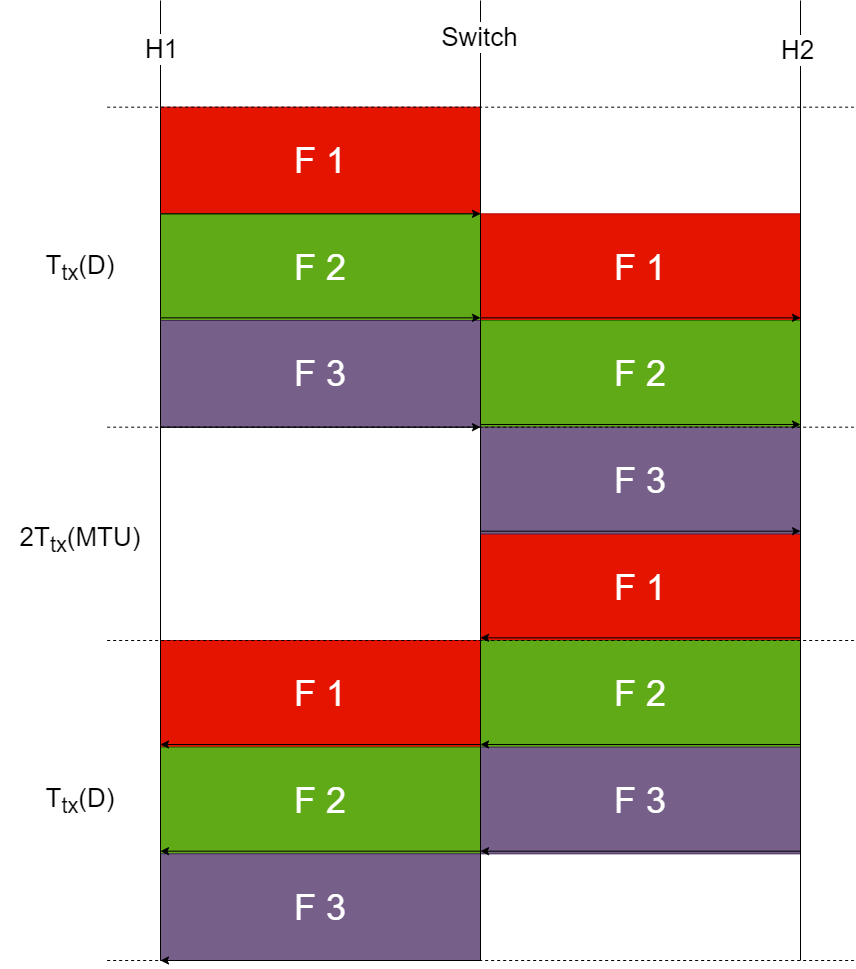
\includegraphics[scale = 0.26]{GraficoSwitch.png}
	\caption{Schema di invio pacchetto con switch}
	\label{fig:GrafSwitch}
\end{figure}

Quando i frammenti diventano più d'uno lo switch, che opera soltanto a livello 2, non è in grado di distinguerli e continua ad operare su di essi separatamente come mostrato in figura \ref{fig:GrafSwitch}.
A seguito della frammentazione la formula per il calcolo del RTT diventa quindi:
 
\begin{equation}
RTT = 2T_{TX}(D) + 2T_{TX}(MTU)
\end{equation}
I tempi di trasmissione del generico dato di dimensione X sono ottenuti come:
\begin{equation}
	T_{TX}(X) = \dfrac{X}{C}
\end{equation}
Facendo uso delle equazioni mostrate sopra otteniamo la funzione della capacità come:
\begin{equation}
	\begin{cases}
		C = \dfrac{4 D }{RTT}, \quad S < 1473 \\
		\\
		C = \dfrac{2D + 2MTU}{RTT} = \dfrac{2D + 2 * 1538}{RTT}, \quad s \geq 1473
	\end{cases}
\end{equation}
\subsection{Velocità: 10Mb/s}
Nel grafico del RTT notiamo che l'andamento è circa lineare e non si discosta di molto da quello ideale. La funzione è definita a tratti come ci aspettiamo dalla formule viste in precedenza. Nel caso del singolo frammento la presenza dello switch ha un effetto negativo(pendenza della retta maggiore) che viene mitigato quando il numero dei frammenti aumenta.

\subsection{Velocià: 100Mb/s}
In questo caso valgono le considerazioni fatte per il precedente caso senza switch(effetto negativo di $\eta$), per quanto riguarda le misure. L'andamento teorico invece è lo stesso del caso precedente a 10 Mbps.







\newpage
\section*{Appendice}
\begin{figure}[H]
	\centering
	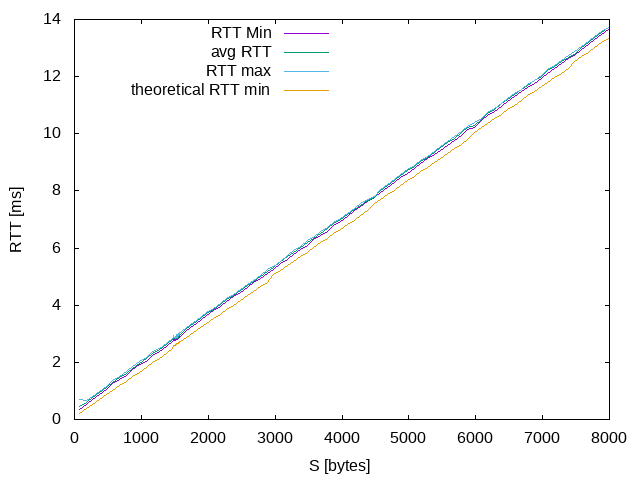
\includegraphics[scale = 0.75]{No_Switch/RTT-10Mbps.png}
	\caption{Grafico Data-RTT senza switch a 10 Mbps}
	\label{fig:2.1RTT}
\end{figure}

\begin{figure}[H]
	\centering
	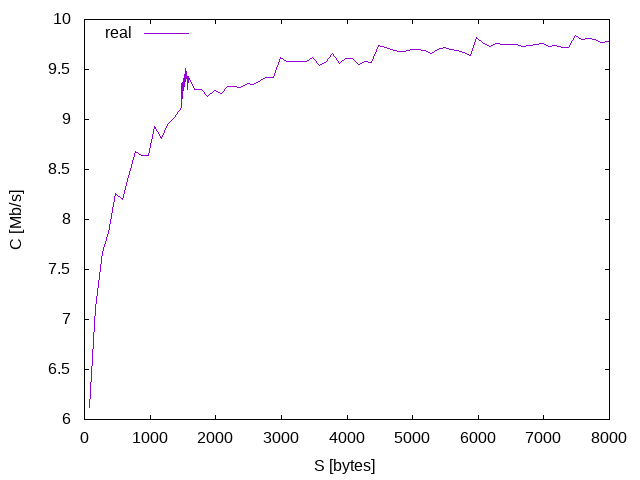
\includegraphics[scale = 0.75]{No_Switch/speed-10Mbps.png}
	\caption{Grafico Dati-Capacità senza switch a 10 Mbps}
	\label{fig:2.1Speed}
\end{figure}

\begin{figure}[H]
	\centering
	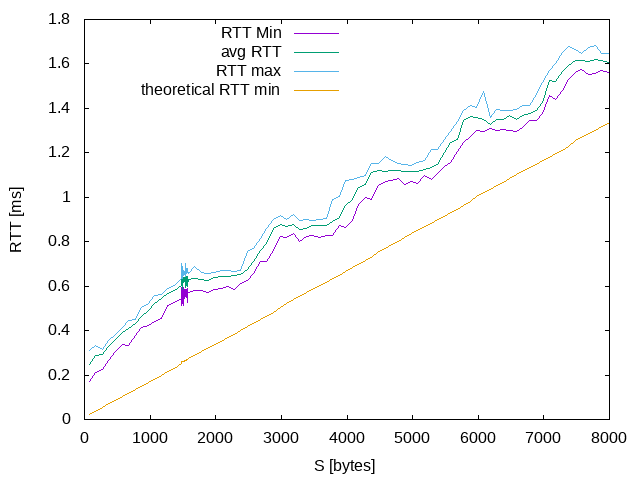
\includegraphics[scale = 0.75]{No_Switch/RTT-100Mbps.png}
	\caption{Grafico Data-RTT senza switch a 100 Mbps}
	\label{fig:2.2RTT}
\end{figure}


\begin{figure}[H]
	\centering
	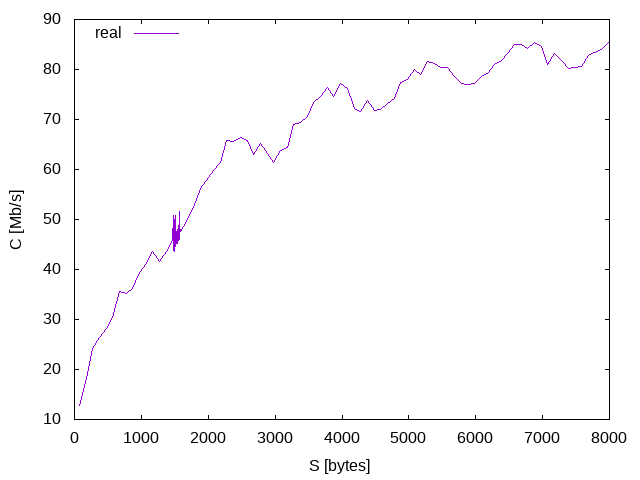
\includegraphics[scale = 0.75]{No_Switch/speed-100Mbps.png}
	\caption{Grafico Data-Capacità senza switch a 100 Mbps}
	\label{fig:2.2Speed}
\end{figure}

\begin{figure}[H]
	\centering
	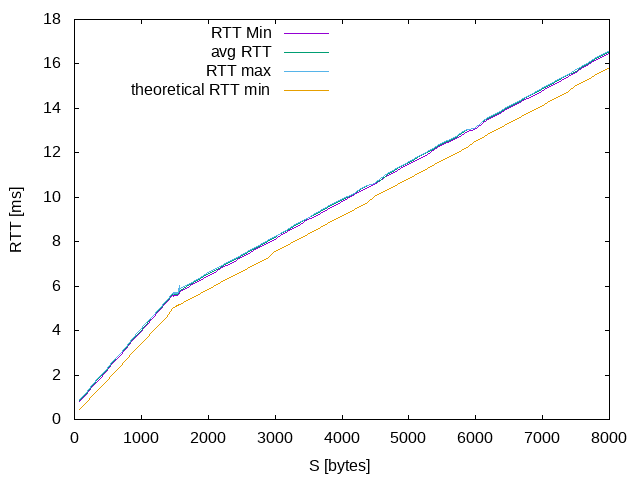
\includegraphics[scale = 0.75]{Si_Switch/RTT-10Mbps.png}
	\caption{Grafico Data-RTT con switch a 10 Mbps}
	\label{fig:3.2RTT}
\end{figure}


\begin{figure}[H]
	\centering
	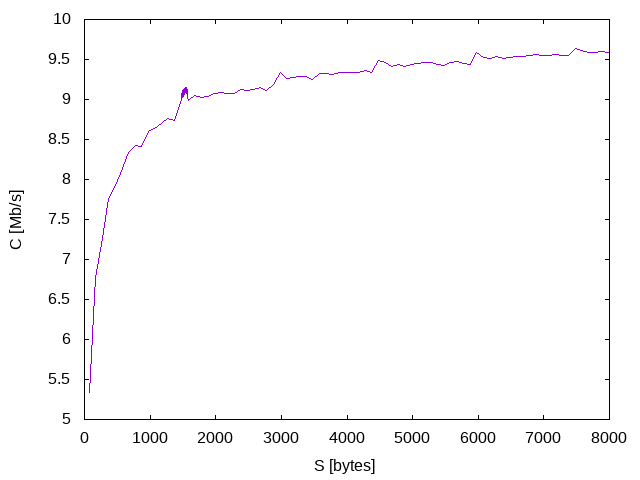
\includegraphics[scale = 0.75]{Si_Switch/speed-10Mbps.png}
	\caption{Grafico Data-Capacità con switch a 10 Mbps}
	\label{fig:3.1Speed}
\end{figure}
\begin{figure}[h!]
	\centering
	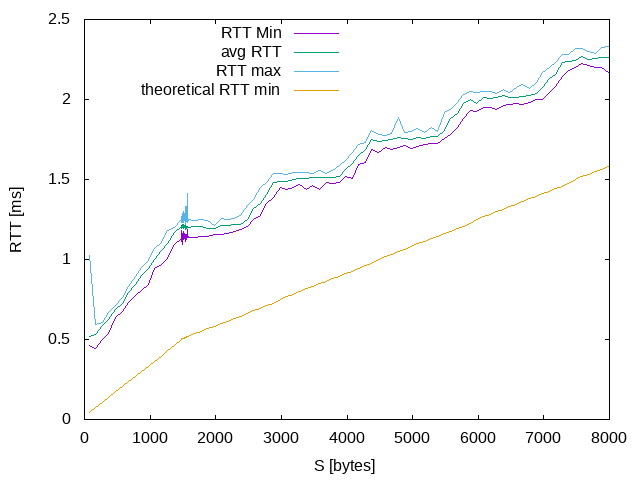
\includegraphics[scale = 0.75]{Si_Switch/RTT-100Mbps.png}
	\caption{Grafico Data-RTT con switch a 100 Mbps}
	\label{fig:3.2RTT}
\end{figure}

\begin{figure}[h!]
	\centering
	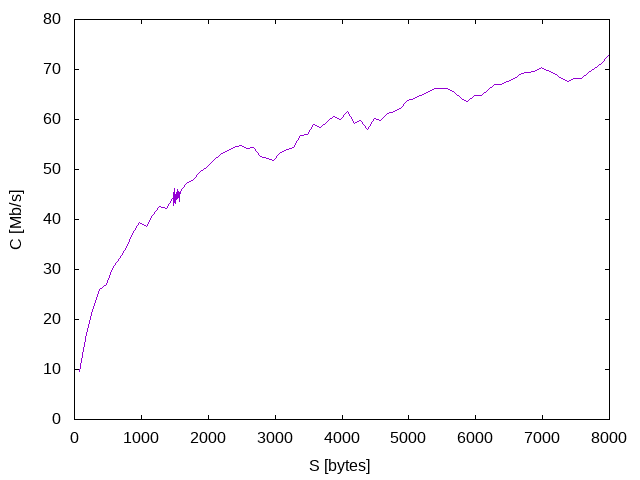
\includegraphics[scale = 0.75]{Si_Switch/speed-100Mbps.png}
	\caption{Grafico Data-Capacità  con switch a 100 Mbps}
	\label{fig:3.2Speed}
\end{figure}


\begin{figure}[h!]
	\centering
	\lstinputlisting[language = bash]{ping.sh}
	\caption{Script per la raccolta dei dati}
	\label{fig:ScriptPing}
\end{figure}

\begin{figure}[]
	\centering
	\lstinputlisting[language=bash]{plot.gnu}
	\caption{Script per generazione grafici in gnuplot a 10Mbps (commentato il caso con lo switch)}
	\label{fig:ScriptPlot}
\end{figure}

\end{document}
